
%%% Local Variables:
%%% mode: latex
%%% TeX-master: t
%%% End:

\chapter{实验与分析}
\label{cha:experiments_analysis}
本章节主要介绍在 Spark 集群上进行近似近邻查询算法的实验,主要包括实验环境介绍、实验数据集介绍、实验结果展示以及实验分析。

下图是 Spark 集群系统的工作模式图。驱动程序(driver)会和集群的管理器(cluster manager)相连接,驱动其为集群其他节点分配资源。在分配完毕以后,驱动程序会将你的应用程序(Scala 中的 jar 包)发送到各个节点的线程池(executor)。之后驱动程序会调配任务给各个节点执行。
\label{cha:experiments_analysis}
\begin{figure}[H]
  \centering
  \includegraphics[width=0.9\linewidth]{spark-yarn}
  \caption{Spark 集群系统工作模式}
  \label{fig:spark-yarn}
\end{figure}
\section{实验环境}
本次实验中关于 Spark 部分的实验都是在由 4 台机器构成的 Spark on YARN 集群系统上完成的。其中,每台机器配置均相同,配置如下:
\begin{itemize}
\item 操作系统:Red Hat Enterprise Linux Server release 7.0
\item 处理器信息:Intel(R) Xeon(R) CPU E5-2609 0 @ 2.40GHz
\item 逻辑核数:8 核
\item 内存大小: 60G
\end{itemize}

关于 MATLAB 部分的实验是在一台单机上完成,配置如下:
\begin{itemize}
\item 操作系统:Windows 8
\item 处理器信息:Intel(R) Core(TM) i3 CPU M 380 @ 2.53GHz
\item 逻辑核数:4 核
\item 内存大小: 6G
\end{itemize}
\section{实验数据集}
实验过程中主要使用到了三个数据集,分别是 SIFT1M\footnote{http://corpus-texmex.irisa.fr/\label{fn:repeat}}、GIST1M\footnotemark[1]、CIFAR-10\footnote{http://www.cs.toronto.edu/~kriz/cifar.html}。 实验主要对比上一章节中介绍的方法在 Spark 集群系统上与 MATLAB 单机系统上的近似近邻查询的召回率以及相应时间消耗,此外也对比在不同的参数下, Spark 集群系统上的运行结果。
\subsection{SIFT1M}
SIFT1M 是近年来被广泛应用于近似近邻查询方法准确率和召回率的衡量。这个数据集中的数据都是 128 维的 SIFT 特征向量,包含三部分:待索引的原始数据集(base)、训练数据集(learn)、查询数据集(query)。其中待索引的原始数据集合有 $10^6$ 个向量,训练数据集有 $10^5$ 个,查询数据集共有 $10^4$ 个。
\subsection{GIST1M}
GIST1M 这个数据集中的数据都是 960 维的 GIST 特征向量,包含三部分:待索引的原始数据集(base)、训练数据集(learn)、查询数据集(query)。其中待索引的原始数据集合有 $10^6$ 个向量,训练数据集有 $5\times10^5$ 个,查询数据集共有 $10^3$ 个。
\subsection{CIFAR-10}
CIFAR-10 数据集被广泛用于在计算机视觉领域做目标识别、图像分类等任务的。它是从 80 million tiny images\footnote{http://groups.csail.mit.edu/vision/TinyImages/} 数据集中挑选出的一个带标签的子集,由 60000 张 $32\times 32$ 的彩色图像组成。它们被分成 10 类,每个类别有 6000 张图片。10 个类别分别是airplane、automobile、bird、cat、deer、dog、frog、horse、ship、truck。

在本次实验中,我们对每张图片提取出 320 维的 GIST 特征表示,这样我们就得到了 60000 个 320 维的 GIST 向量。我们从中选取 1000 个作为查询数据,剩余的作为训练数据和待检索数据集。在编码数据集上进行近似近邻查询出前 500 张图片,根据原有的类别标签来衡量查询的准确率。

\begin{figure}[H]
  \centering
  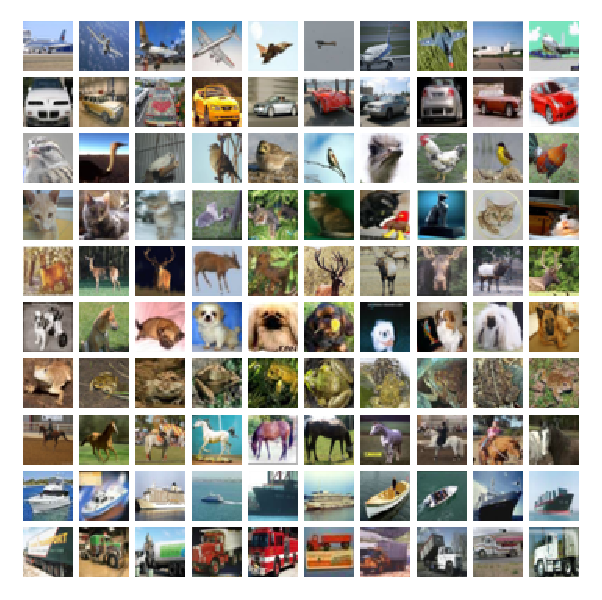
\includegraphics[width=0.7\linewidth]{cifar-10}
  \caption{CIFAR-10 数据集中图片示例}
  \label{fig:cifar-10}
\end{figure}
\section{实验结果与分析}
\subsection{SIFT1M 对比实验}
本实验室在 SIFT1M 数据上进行,通过比较 Spark 集群上的乘积量化的近似近邻查询方法与同样方法在 MATLAB 单机上的实验的召回率和时间消耗的对比。

在 Spark 集群系统上的程序参数设置,我们采用 yarn-client 模式在集群上运行程序,设置 executor 的数量为 40,每一个 executor 的内存大小限制为 5G。在对 SIFT1M 数据集近似近邻查询实验中,我们设置子空间切分数量 $m$ 为 8,子空间中的聚类中心数量为 $h$ 为 256,因此总的聚类中心的数量就是 $2^{64}$,编码字节的大小就是 64 比特。$h$ 取 256 是比较合适的,恰当的子空间聚类中心数量一方面可以使得查找表的大小不会过大,另一方面保证训练和编码的时间也不会太长。在这次实验中,我们采用 recall@$R$ 作为查询效果好坏的衡量标准,其中 $R$ 是检出数据集的大小。SIFT1M 数据中有 $10^4$ 个查询向量,对于一个查询向量,通过整个近似近邻查询计算,我们在原始向量中找到前 100 个近邻向量,并分别取 $R$ 为 1、2、5、10、20、50、100,计算前 $R$ 个向量中出现最近邻向量的次数 $s$,那么衡量标准就可以由公式 recall@$R = s/10^4$ 计算得出。
\begin{table}[htbp]
\noindent\begin{minipage}{0.5\textwidth}
\centering
\caption{Spark 与 MATLAB 上召回率对比}
\label{tab:recall_on_spark_matlab}
\begin{tabular}{ccc}
\toprule[1.5pt]
    & Spark & MATLAB\\
  \hline
  recall@1  &  0.23   & 0.29\\
  recall@2  &  0.33 &   0.40\\
  recall@5  &  0.48 &   0.53\\
  recall@10  & 0.60 &   0.62\\
  recall@20  &  0.72&  0.73\\
  recall@50  &  0.85 &  0.81\\
  recall@100  & 0.92 &  0.88\\
\bottomrule[1.5pt]
    \end{tabular}
\end{minipage}
\begin{minipage}{0.5\textwidth}
\centering
\caption{Spark 与 MATLAB 上时间对比}
\label{tab:time_on_spark_matlab}
\begin{tabular}{ccc}
\toprule[1.5pt]
    & Spark & MATLAB \\
\hline
训练时间(s) & 1193.04 & 1574.09  \\
编码时间(s) & 12.42 & 49.93 \\
单次查询时间(s)& 2.89 & 181.71 \\
\bottomrule[1.5pt]
\end{tabular}
\end{minipage}
\end{table}
表 \ref{tab:recall_on_spark_matlab} 和表 \ref{tab:time_on_spark_matlab} 分别显示的是在 Spark 上与 MATLAB 中的召回率对比以及所用时间对比。仅从表 \ref{tab:recall_on_spark_matlab} 来看,Spark 集群系统上程序的召回率与 MATLAB 单机版本的相差不大。在保证召回率差不多的情况下,我们再看表  \ref{tab:time_on_spark_matlab},从表中我们可以看出在训练阶段的时间消耗上,Spark 比 MATLAB 耗时要少,但是并没有成倍数减少。在编码阶段时间消耗, Spark 集群上用时仅为 MATLAB 的 $1/4$ 左右。到了查询阶段,单次耗时 MATLAB 是 Spark 集群系统上单次耗时的 $70$ 余倍。
\subsection{GIST1M 实验}
对 GIST1M 数据集的实验都在 Spark 集群系统上完成, Spark 集群系统的配置上面的实验相同,在 yarn-client 模式执行程序, executor 的数量为 40,executor 的内存大小限制为 5G。 在本次实验中,我们分别采用 32 比特、64 比特、96 比特、128比特、256 比特这些不同编码长度进行实验,观察实验中 recall@$R$ 的变化,$R$ 是检出数据集大小。
\begin{figure}[H]
  \centering
  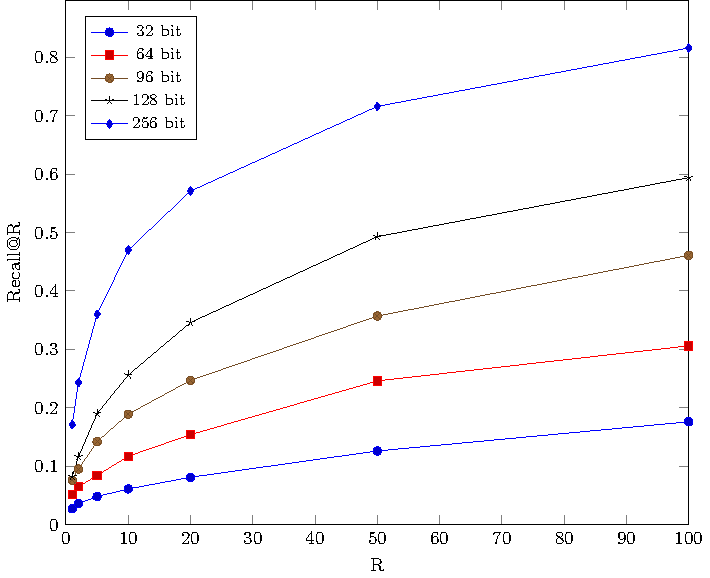
\includegraphics[width=0.6\linewidth]{gist}
  \caption{GIST1M 上不同编码长度下的召回率对比}
  \label{fig:gist}
\end{figure}
从上图 \ref{fig:gist} 中可以看出,在同等检出数量下,编码长度越长,召回率越高。由此,也可以证明算法的正确性。
\subsection{CIFAR-10 实验}
在 CIFAR-10 数据集上的实验中,Spark 集群系统的配置以及程序的参数设置和 GIST1M 中完全相同。分别对不同长度的编码进行对比实验,根据数据集原有的类别标签,我们采用准确率 precision 来衡量检出效果,图中 $R$ 是检出数据的数量。
\begin{figure}[H]
  \centering
  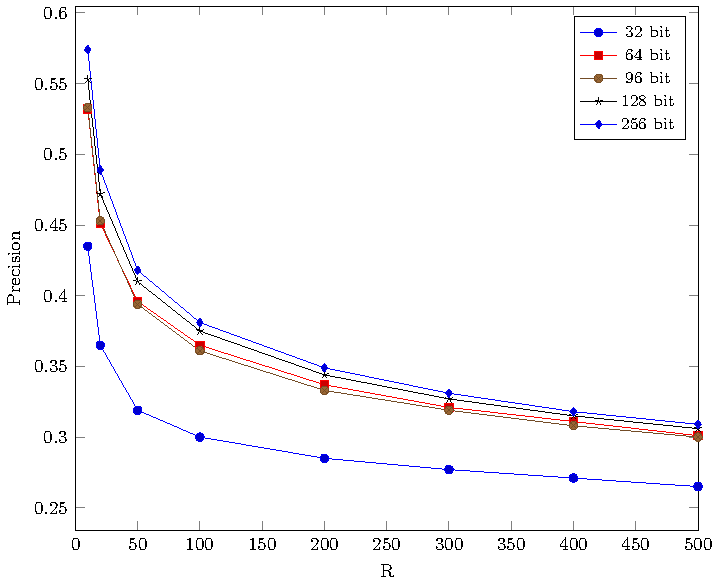
\includegraphics[width=0.6\linewidth]{cifar-result}
  \caption{CIFAR-10 上不同编码长度下的查准率对比}
  \label{fig:cifar-result}
\end{figure}
从图 \ref{fig:cifar-result} 中,我们可以看到在同样的压缩编码下,准确率随着检出数量增大而不断降低。在相同的检出数量条件下,编码长度越长,检出的准确率越高。下图 \ref{fig:horse} 是实验中对于一个查询图片检索出前 25 个相似图片的示例。
\begin{figure}[H]
  \centering
  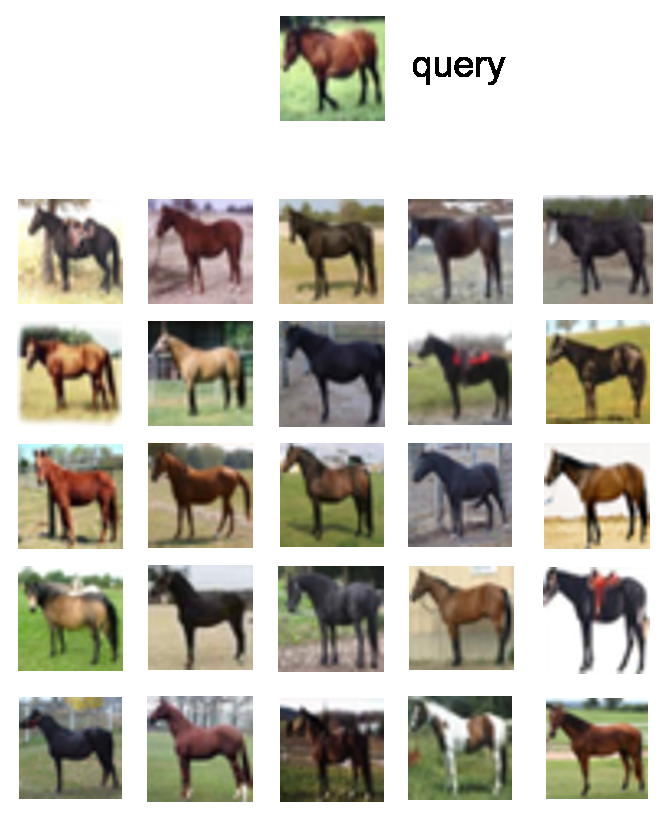
\includegraphics[width=0.5\linewidth]{horse}
  \caption{CIFAR-10 数据集上图像查询实例}
  \label{fig:horse}
\end{figure}
\subsection{本章小结}
本章中主要介绍了在 SIFT1M、GIST1M、CIFAR-10 三个数据集上分别进行实验。在 SIFT1M 数据集上,通过对比 Spark 集群系统上 和 MATLAB 上的召回率以及查询时间,可以看出 我们的近似近邻查询系统的正确性以及查询效率的加速情况。在 GIST1M 上的实验说明,我们系统有比较好的扩展性,同时结果也表明了查询系统的正确性。在 CIFAR-10 数据集上的实验表明我们的系统能够应用于大规模图像检索当中。
